%% 
%% Copyright 2019-2024 Elsevier Ltd
%% 
%% This file is part of the 'CAS Bundle'.
%% --------------------------------------
%% 
%% It may be distributed under the conditions of the LaTeX Project Public
%% License, either version 1.3c of this license or (at your option) any
%% later version.  The latest version of this license is in
%%    http://www.latex-project.org/lppl.txt
%% and version 1.3c or later is part of all distributions of LaTeX
%% version 1999/12/01 or later.
%% 
%% The list of all files belonging to the 'CAS Bundle' is
%% given in the file `manifest.txt'.
%% 
%% Template article for cas-sc documentclass for 
%% double column output.

\documentclass[a4paper]{cas-sc}
\usepackage{amssymb}
%% The amsmath package provides various useful equation environments.
\usepackage{amsmath}
\usepackage{multirow}
\usepackage{algorithm}
\usepackage{algpseudocode}
\usepackage{booktabs}
\usepackage{graphicx}
\usepackage{xcolor}

% Revision marker: every \TODO must be resolved from the re-run results before submission.
% Set \revisionfalse to hide them in a draft for co-authors (they must still be resolved).
\newif\ifrevision \revisiontrue
\newcommand{\TODO}[1]{\ifrevision\textcolor{red}{[TODO: #1]}\fi}





% If the frontmatter runs over more than one page
% use the longmktitle option.

%\documentclass[a4paper,fleqn,longmktitle]{cas-sc}

%\usepackage[numbers]{natbib}
%\usepackage[authoryear]{natbib}
\usepackage[numbers]{natbib}

%%%Author macros
\def\tsc#1{\csdef{#1}{\textsc{\lowercase{#1}}\xspace}}
\tsc{WGM}
\tsc{QE}
%%%

% Uncomment and use as if needed
%\newtheorem{theorem}{Theorem}
%\newtheorem{lemma}[theorem]{Lemma}
%\newdefinition{rmk}{Remark}
%\newproof{pf}{Proof}
%\newproof{pot}{Proof of Theorem \ref{thm}}

\begin{document}
\let\WriteBookmarks\relax
\def\floatpagepagefraction{1}
\def\textpagefraction{.001}
% Short title
\shorttitle{DEGST: Dynamic Entropy-Guided Sparse Training}    

\shortauthors{Ha Vu et al.}  

% Main title of the paper
\title [mode = title]{Dynamic Entropy-Guided Sparse Training for Efficient Neural Network Compression}  



% First author
\author[label1]{Minh-Duc Ha Vu}
\credit{Conceptualization, Methodology, Software}
\ead{havuminhduc_t67@hus.edu.vn}

\author[label1]{Bao Phan Dinh Thai}
\credit{Methodology, Validation}
\ead{phandinhthaibao_t67@hus.edu.vn}

\author[label2]{Hung Tran Duy}
\credit{Validation, Investigation}
\ead{24021506@vnu.edu.vn}

\author[label3]{Quyen Quach Thai}
\credit{Formal analysis, Investigation \& review}
\ead{quyenqt@vnu.edu.vn}

\author[label3]{Hai Le Xuan}
\credit{Data curation \& reivew}
\ead{hailx@vnu.edu.vn}

\author[label3]{Van-Tien Giap\cormark[1]}
\credit{Supervision, Writing - review \& editing}
\ead{tiengv@vnu.edu.vn}

\cortext[1]{Corresponding author}

% Affiliations
\affiliation[label1]{organization={VNU University of Science},
            city={Hanoi},
            country={Vietnam}}

\affiliation[label2]{organization={VNU University of Engineering and Technology},
            city={Hanoi},
            country={Vietnam}}

\affiliation[label3]{organization={VNU International School},
            city={Hanoi},
            country={Vietnam}}


% For a title note without a number/mark
%\nonumnote{}

% Here goes the abstract
\begin{abstract}
Dynamic sparse training methods such as RigL update the sparse topology during training, dropping connections by weight magnitude and regrowing them by gradient magnitude. We ask whether the entropy of the activations a weight reads adds useful information to the drop decision. Dynamic Entropy-Guided Sparse Training (DEGST) scores each weight by the histogram entropy of its input channel multiplied by its magnitude, $H(A)\cdot|w|$, inside an otherwise standard prune-and-regrow loop. A channel-level variant, DEGST-S, applies the entropy score to coupled channel groups and removes the selected channels physically, and a hybrid variant combines both levels under one weight budget.

To isolate the contribution of entropy, we keep the training loop fixed and change only the drop criterion ($|w|$, $H(A)$, $H(A)\cdot|w|$). We then compare against RigL, gradual magnitude pruning, SNIP, movement pruning, Network Slimming, FPGM and an AutoPruner-style baseline. All methods keep the same number of weights, share one training recipe without method-specific tuning, and are run with three seeds at the main operating points. Accuracy is plotted against both non-zero and actually executed FLOPs, on CIFAR-10 with ResNet-18, with additional runs on CIFAR-100 and on MobileNetV2.

\TODO{State the C0 outcome in one sentence with numbers, e.g. ``At 90\% sparsity on CIFAR-10, $H(A)\cdot|w|$ changes accuracy by $X\pm Y$ points relative to $|w|$ in the same loop'', and say plainly whether this exceeds seed variance.} \TODO{State where DEGST, DEGST-S and the hybrid lie relative to the Pareto front at equal FLOPs, naming any baseline that dominates them.} Unstructured sparsity, including that of DEGST, gives no measurable speed-up with dense GPU kernels; only the channel-level variants reduce latency.
\end{abstract}

% Use if graphical abstract is present
%\begin{graphicalabstract}
%\includegraphics{}
%\end{graphicalabstract}

% Research highlights
% \begin{highlights}
% \item DEGST introduces entropy-guided dynamic sparse training.
% \item Global prune-regrow enables adaptive topology optimization.
% \item A unified criterion bridges unstructured and structured pruning.
% \item Hybrid sparsity improves deployment efficiency and throughput.
% \item Experiments explore the accuracy-efficiency trade-offs across different structural granularities.
% \end{highlights}


% Keywords
% Each keyword is seperated by 
\begin{keywords}
 Dynamic sparse training\sep Neural network pruning\sep Activation entropy\sep Structured sparsity\sep Unstructured sparsity\sep Model compression
\end{keywords}



\maketitle

% Main text
\section{Introduction}
\label{sec:intro}

Deep neural networks (DNNs) achieve strong performance across computer vision \cite{he2016deep,dosovitskiy2020image}, but this performance comes with high computational cost, large parameter counts and substantial memory demand \cite{hoefler2021sparsity}. These costs make deployment difficult on mobile, embedded and edge devices \cite{howard2017mobilenets,ma2018shufflenet}. Model compression addresses this through quantization \cite{jacob2018quantization}, knowledge distillation \cite{hinton2015distilling}, efficient architecture design \cite{tan2019efficientnet} and network pruning \cite{han2015learning,blalock2020state}. Pruning is attractive because it reduces parameters and computation of an existing architecture while preserving much of its accuracy \cite{liu2018rethinking}.

Classical pruning estimates the importance of each weight after dense training, either from the loss curvature, as in Optimal Brain Damage and Optimal Brain Surgeon \cite{lecun1989optimal,hassibi1992second}, or from weight magnitude \cite{han2015learning}, and then fine-tunes the pruned network \cite{liu2017learning}. Because this train--prune--fine-tune pipeline is expensive, \emph{sparse training} methods learn the sparse network during a single training run. Some fix the mask at initialisation \cite{lee2018snip,wang2020picking,tanaka2020synflow}, others prune gradually during training \cite{zhu2017prune,sanh2020movement}, and \emph{dynamic sparse training} (DST) methods keep the sparsity constant while periodically dropping and regrowing connections \cite{mocanu2018scalable,bellec2017deep,mostafa2019parameter,dettmers2019sparse,evci2020rigging}. In the most widely used DST method, RigL \cite{evci2020rigging}, connections are dropped by weight magnitude and regrown by gradient magnitude.

Magnitude says nothing about the signal a weight multiplies. A large weight attached to an input channel that is almost constant over the data contributes little beyond a bias, whereas a moderate weight on a channel with a wide, input-dependent distribution takes part in many different responses. Activation statistics have long been used to choose \emph{channels} to prune: the fraction of zero activations \cite{hu2016network}, the entropy of pooled channel responses \cite{luo2017entropy}, feature-map rank \cite{lin2020hrank} and channel independence \cite{sui2021chip}. We are not aware of work that evaluates them as the \emph{drop criterion of a DST loop}, where the score is recomputed many times during training and interacts with gradient-based regrowth. \TODO{Confirm this with a literature search (2022--2025 DST papers) before submission.}

This paper tests that idea. We propose Dynamic Entropy-Guided Sparse Training (DEGST), which estimates the histogram entropy $H(A)$ of each input channel from the training batches preceding a topology update, scores each weight by $H(A)\cdot|w|$, and otherwise follows a standard prune-and-regrow loop. Because the same entropy estimate is defined per channel, it also yields a channel score. We use it in DEGST-S, which prunes and regrows coupled channel groups and removes them physically, and in a hybrid variant that splits one weight budget between channel removal and unstructured sparsity.

A drop criterion that combines entropy with magnitude can only be credited to entropy if it beats magnitude alone under otherwise identical conditions. We therefore design the evaluation around three controls. First, an ablation runs the same loop with $|w|$, $H(A)$ and $H(A)\cdot|w|$ as the only difference. Second, all methods, including RigL, are compared at the same weight budget, with one shared training recipe and three seeds. Third, accuracy is reported against FLOPs rather than against nominal sparsity. The third control matters because methods that allocate sparsity globally prune late, low-resolution layers hardest: at equal parameter sparsity they remove far fewer FLOPs than layer-uniform methods, and a comparison at equal sparsity would mix two different operating regimes. We also report executed FLOPs and measured latency separately from non-zero FLOPs, because unstructured sparsity does not accelerate dense GPU kernels \cite{gale2020sparse,elsen2020fast,hoefler2021sparsity}.

The contributions of this paper are:
\begin{itemize}
    \item DEGST, a dynamic sparse training method whose drop criterion weights magnitude by the entropy of the input activation, with channel-level (DEGST-S) and hybrid variants that share the entropy estimate and remove channels physically using dependency-graph pruning \cite{fang2023depgraph}.
    \item A controlled ablation that separates the contribution of entropy from that of the prune-and-regrow loop, together with a comparison of further criteria (Taylor, Fisher, gradient, movement) inside the same loop.
    \item An evaluation at matched weight budgets on CIFAR-10 with ResNet-18, complemented by CIFAR-100 and MobileNetV2. It reports accuracy--FLOPs Pareto fronts for both non-zero and executed FLOPs, a documented latency/throughput protocol, training cost and hyper-parameter sensitivity.
    \item \TODO{One sentence summarising the main empirical finding, stated plainly (positive or negative), once C0 and the Pareto sweep are complete.}
\end{itemize}

\section{Related Work}
\label{sec:related}

\paragraph{Pruning after training.}
Removing weights by loss curvature \cite{lecun1989optimal,hassibi1992second} or by magnitude \cite{han2015learning} showed early on that trained networks are highly redundant. Later work refined the saliency estimate with first-order Taylor expansions \cite{molchanov2017pruning,molchanov2019importance}, empirical Fisher information \cite{theis2018faster} and layer-wise second-order reconstruction \cite{frantar2022obc}. These criteria estimate the increase in loss caused by removing a weight, which is the quantity pruning ultimately needs to control. Large-scale comparisons \cite{gale2019state,blalock2020state,hoefler2021sparsity} found that careful magnitude pruning remains a strong baseline and that many reported gains disappear under matched training budgets, a finding that motivates the controls in this paper.

\paragraph{Pruning at initialisation and gradual pruning.}
SNIP \cite{lee2018snip}, GraSP \cite{wang2020picking} and SynFlow \cite{tanaka2020synflow} fix a mask before training from connection sensitivity or gradient flow; random masks with appropriate layer-wise densities are competitive with them \cite{liu2022random}. Gradual magnitude pruning (GMP) \cite{zhu2017prune} increases sparsity along a cubic schedule during training. Movement pruning \cite{sanh2020movement} keeps weights that move away from zero during training, and dynamic pruning with feedback \cite{lin2020dpf} lets pruned weights recover. The lottery-ticket line of work \cite{frankle2018the,renda2020comparing} studies which sparse sub-networks train well from (near) initialisation.

\paragraph{Dynamic sparse training.}
DST keeps the parameter count fixed throughout training and periodically rewires the network. SET \cite{mocanu2018scalable} drops the smallest-magnitude weights and regrows at random, DeepR \cite{bellec2017deep} rewires stochastically, and DSR \cite{mostafa2019parameter} reallocates parameters across layers. SNFS \cite{dettmers2019sparse} regrows by momentum. RigL \cite{evci2020rigging} regrows by instantaneous gradient magnitude, uses an Erd\H{o}s--R\'enyi-kernel (ERK) layer allocation and decays the update fraction with a cosine schedule; it is the reference DST method and our closest baseline. Subsequent work studied why DST works, attributing it to parameter exploration over time \cite{liu2021itop} and to improved gradient flow \cite{evci2022gradient}. Other work combined DST with gradual pruning \cite{liu2021granet}, kept backward passes sparse as well \cite{jayakumar2020topkast}, targeted memory-limited edge training \cite{yuan2021mest} or learned layer-wise thresholds \cite{kusupati2020soft}. Nearly all of these methods drop by magnitude and change the \emph{regrowth} rule or the schedule. DEGST changes the \emph{drop} rule and keeps RigL's gradient regrowth, so our ablation can attribute any difference to the drop criterion alone.

\paragraph{Structured pruning and activation-based channel selection.}
Structured methods remove whole filters or channels so that the result is a smaller dense network. They score channels by filter norms \cite{li2016pruning}, BatchNorm scaling factors trained under an $\ell_1$ penalty (Network Slimming) \cite{liu2017learning}, distance to the geometric median of a layer's filters (FPGM) \cite{he2019filter}, reconstruction error of the next layer \cite{luo2017thinet,he2017channel}, importance propagated from the output \cite{yu2018nisp}, or learned channel gates (AutoPruner) \cite{luo2020autopruner}. Soft filter pruning \cite{he2018soft} lets pruned filters recover during training, and group-sparsity regularisation \cite{wen2016learning} learns structure directly. Several methods score channels with \emph{activation} statistics: the average percentage of zeros \cite{hu2016network}, the entropy of globally pooled channel responses \cite{luo2017entropy}, the rank of feature maps \cite{lin2020hrank} and the independence between channels \cite{sui2021chip}. DEGST-S uses a per-channel histogram entropy in the same spirit, but inside a prune-and-regrow loop rather than a one-shot selection. In residual and depthwise architectures, channels are coupled across layers; we use DepGraph \cite{fang2023depgraph} to find the coupled groups and to remove them physically.

\paragraph{Information-theoretic views of representations.}
The information bottleneck view of deep learning \cite{tishby2015deep,shwartz2017opening} motivates entropy as a descriptor of how much a representation varies with the input. A caveat applies to all entropy-based criteria, including ours: a channel's marginal entropy measures the diversity of its values, not the sensitivity of the loss to removing the weights that read it. Low entropy suggests redundancy but does not establish it, which is why we compare entropy-based scores directly with loss-sensitivity scores (Taylor and Fisher) in the same loop.

\paragraph{Hardware efficiency of sparsity.}
Irregular sparsity is difficult to accelerate on GPUs. Speed-ups need specialised sparse kernels at high sparsity \cite{gale2020sparse,elsen2020fast} or constrained patterns such as 2:4 semi-structured sparsity supported by recent tensor cores \cite{mishra2021accelerating,zhou2021nm}. Structured pruning reduces latency on standard dense kernels. We therefore report non-zero FLOPs, executed FLOPs and measured latency separately.

\section{Method}
\label{sec:methods}

DEGST trains a sparse network in a single run. After a short dense warm-up, a sparse mask is initialised, and every $\Delta T$ iterations a fraction of the active weights is dropped according to an entropy-weighted score and replaced by the same number of inactive weights with the largest gradient. The loop is the one of RigL \cite{evci2020rigging}; the drop score and the mask initialisation are what DEGST changes (Algorithm~\ref{alg:degst}, Fig.~\ref{fig:framework}). Sections~\ref{sec:degst-s} and~\ref{sec:hybrid} extend the same entropy estimate to channels.

\begin{figure}
    \centering
    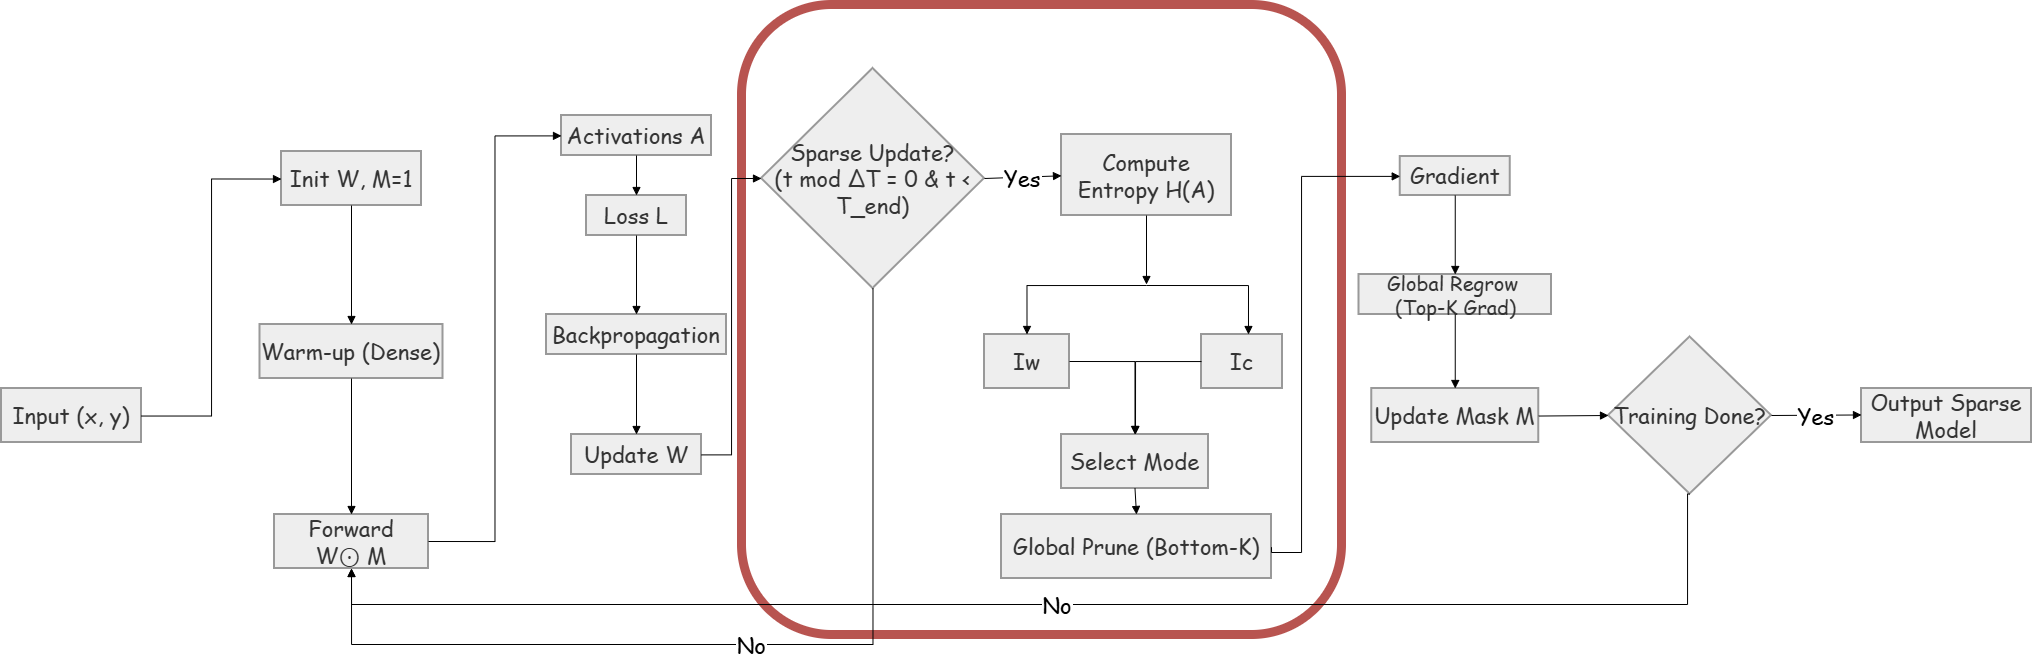
\includegraphics[width=1\linewidth]{Figures/Pipeline_highlight.png}
    \caption{DEGST training loop. After a dense warm-up, the entropy-guided branch (highlighted) runs every $\Delta T$ iterations until $T_{\text{end}}$: activation entropy is estimated from recent training batches and turned into weight-level ($I_w$) or channel-level ($I_c$) scores, the lowest-scoring active elements are dropped globally, and the same number of inactive elements with the largest gradient are regrown.}
    \label{fig:framework}
\end{figure}

\subsection{Notation and sparsity budget}

Let $W$ collect the weights of all convolutional and linear layers, $N=|W|$, and let $M\in\{0,1\}^{N}$ be a binary mask. The network computes with $W\odot M$ and is trained on the usual empirical risk. Throughout the paper, the \emph{sparsity} of a model is
\begin{equation}
S = 1 - \frac{\#\{\text{non-zero conv/linear weights of the final model}\}}{N},
\label{eq:sparsity}
\end{equation}
where $N$ always refers to the \emph{dense} model. Channels that are removed physically count as zeros. All methods, whether unstructured, structured or hybrid, are compared at the same $S$ and therefore keep the same number of weights. BatchNorm parameters are excluded from $N$; their count is reported separately.

\subsection{Activation entropy}

For a prunable layer $l$ with input tensor $A^{(l)}\in\mathbb{R}^{n\times C\times H\times W}$, we treat the $nHW$ values of input channel $c$ in a mini-batch as samples of a scalar random variable. Its range $[\min, \max]$ in that mini-batch is divided into $B$ equal-width bins. With $p_k$ the fraction of values that fall into bin $k$,
\begin{equation}
H^{(l)}_c = -\sum_{k=1}^{B} p_k \log (p_k + \epsilon),
\label{eq:entropy}
\end{equation}
with $B=30$ and $\epsilon=10^{-8}$. A channel that is constant over the batch has $H=0$, and the maximum is $\log B$. The estimate is taken from the last $K=4$ \emph{training} mini-batches before each topology update, with forward hooks, so no additional forward passes are needed. The $K$ values are aggregated by their mean (the median is evaluated in Sec.~\ref{sec:sensitivity}). For linear layers the samples are the $n$ values of each input feature.

A weight $w$ of layer $l$ reads exactly one input channel $c(w)$. For a grouped convolution with $G$ groups, output channel $o$ and in-group index $i$ read channel $\lfloor o/(C_{\text{out}}/G)\rfloor\cdot C_{\text{in}}/G + i$. The weight therefore inherits $H(w) := H^{(l)}_{c(w)}$ (Fig.~\ref{fig:entropy}).

\begin{figure}
    \centering
    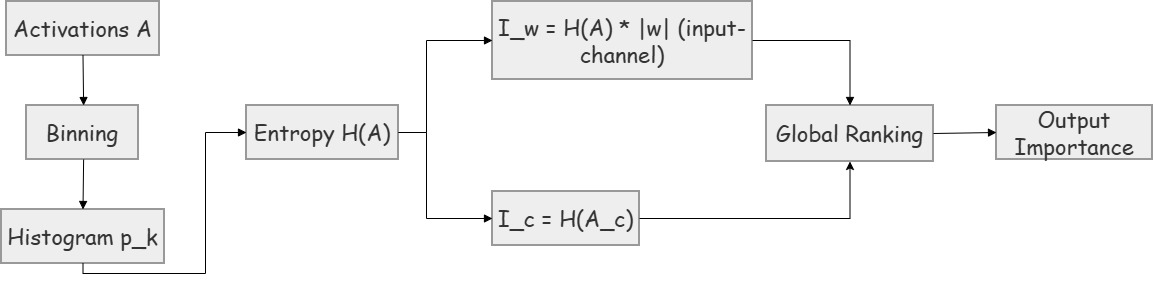
\includegraphics[width=0.75\linewidth]{Figures/Fig.2.jpg}
    \caption{Entropy-guided importance. Activations of each input channel are binned into a histogram, whose entropy is assigned to every weight that reads that channel ($I_w = H(A)\cdot|w|$). For channel pruning, the entropy of a channel's normalised output gives $I_c$. Both scores are ranked globally.}
    \label{fig:entropy}
\end{figure}

\paragraph{What entropy does and does not measure.}
Low $H$ means the input channel takes few distinct values over the data, for example a ReLU channel that is almost always zero or a saturated one. A weight reading such a channel acts almost like a bias, which motivates down-weighting it. However, $H$ is a property of the input distribution, not of the loss. It does not estimate how much the loss increases when the weight is removed, which is the quantity Taylor or Fisher saliencies approximate \cite{molchanov2019importance,theis2018faster}. Whether entropy helps is therefore an empirical question, and Sec.~\ref{sec:c0} answers it with an ablation.

\subsection{DEGST: entropy-weighted drop, gradient regrowth}
\label{sec:degst}

\paragraph{Scores.} The drop score of an active weight is
\begin{equation}
I_w = H(w)\cdot |w|.
\label{eq:iw}
\end{equation}
In the ablation of Sec.~\ref{sec:c0}, this score is replaced by $|w|$ (configuration A, the RigL drop criterion) or by $H(w)$ alone (configuration B), with everything else unchanged.

\paragraph{Mask initialisation.} The network is trained densely for $T_w$ epochs. The mask is then set by keeping the $(1-S)N$ weights with the largest $I_w$, ranked globally across layers.

\paragraph{Prune and regrow.} At every update step $t\in(T_w, T_{\text{end}}]$ with $t \bmod \Delta T = 0$, a fraction
\begin{equation}
\alpha_t = \frac{\alpha}{2}\left(1+\cos\frac{\pi (t-T_w)}{T_{\text{end}}-T_w}\right)
\label{eq:alpha}
\end{equation}
of the currently active weights is updated \cite{evci2020rigging}. The $k=\lfloor \alpha_t\, \|M\|_0\rfloor$ active weights with the smallest $I_w$ are dropped. The ranking is global, but the top 1\% of each layer's active weights are exempt so that no layer is disconnected. The same number of weights that were inactive before the update are regrown, choosing those with the largest dense gradient magnitude $|\partial\mathcal{L}/\partial w|$ on the current mini-batch. Regrown weights start at zero, and the momentum of every changed position is reset. Between updates, gradients of inactive weights are zeroed before the optimiser step, so the sparsity stays exactly $S$. Ties are broken by parameter index (stable sort), which makes the update deterministic given the scores.

\paragraph{Global versus per-layer allocation.} Because the ranking is global, the per-layer density is not fixed in advance: it emerges from the scores. Global magnitude-type rankings keep proportionally more weights in early layers, which operate at high spatial resolution. At a given $S$, they therefore remove fewer FLOPs than a layer-uniform allocation. This is why Sec.~\ref{sec:results} compares methods at equal FLOPs as well as at equal $S$.

\begin{algorithm}
\caption{DEGST (unstructured)}
\label{alg:degst}
\begin{algorithmic}[1]
\Require data $\mathcal{D}$, weights $W$, target sparsity $S$, warm-up $T_w$, interval $\Delta T$, end $T_{\text{end}}$, update fraction $\alpha$
\State $M \gets \mathbf{1}$
\For{$t = 1,\dots,T$}
\State forward with $W\odot M$ \Comment{hooks record $H^{(l)}_c$ if an update is due within $K$ steps}
\State backward: dense gradient $g$
\If{$t = T_w$}
\State $M \gets$ top-$(1-S)N$ of $I_w = H\cdot|w|$ (global)
\ElsIf{$T_w < t \le T_{\text{end}}$ \textbf{and} $t \bmod \Delta T = 0$}
\State $k \gets \lfloor \alpha_t \|M\|_0 \rfloor$ \Comment{Eq.~(\ref{eq:alpha})}
\State drop the $k$ active weights with smallest $I_w$ (global, per-layer floor)
\State grow the $k$ previously inactive weights with largest $|g|$; set them to $0$; reset their momentum
\EndIf
\State $g \gets g \odot M$; SGD step; $W \gets W\odot M$
\EndFor
\State \Return $W\odot M$
\end{algorithmic}
\end{algorithm}

\subsection{DEGST-S: channel-level prune and regrow}
\label{sec:degst-s}

\paragraph{Coupled channel groups.} In residual networks, the channels of the residual stream are shared by the stem, by the last convolution of every block and by the shortcut projections. In MobileNetV2, the expansion and depthwise convolutions are coupled as well. Such channels can only be removed together. We obtain the coupled groups from DepGraph \cite{fang2023depgraph}: ResNet-18 has 12 groups and MobileNetV2 has 26. The classifier's output is never pruned.

\paragraph{Gates.} Each group $g$ carries a binary gate vector that multiplies the outputs of all BatchNorm layers in the group. A zero gate silences the channel everywhere it appears, so the gated network is exactly equivalent to the network with that channel removed. We verified that the outputs agree to $10^{-7}$ after physical removal. The gate also provides a regrowth signal: its gradient $\partial\mathcal{L}/\partial g_c$ is defined for silenced channels, which lets channels be regrown in the same way that RigL regrows weights.

\paragraph{Channel score and schedule.} The channel score $I_c$ is the entropy (Eq.~\ref{eq:entropy}) of the channel's BatchNorm output, averaged over the BatchNorm layers of its group. The weight budget follows the cubic schedule of \cite{zhu2017prune}, from $N$ at $T_w$ to $(1-S)N$ at $T_{\text{end}}$. At each update, a fraction $\alpha_t$ of the active channels with the smallest $I_c$ is swapped for the inactive channels with the largest $|\partial\mathcal{L}/\partial g_c|$ accumulated since the previous update. The lowest-$I_c$ channels are then silenced, in global order, until the weight count computed for the resulting architecture reaches the scheduled budget. Every group keeps at least 5\% of its channels. At $T_{\text{end}}$ the silenced channels are removed physically, and training continues on the compact dense model. The final weight count matches the budget to within one channel.

\subsection{Hybrid sparsity}
\label{sec:hybrid}

The hybrid variant splits one budget $S$ between the two levels. The structured stage runs DEGST-S towards a weight sparsity $\beta S$ ($\beta=0.5$ by default) and removes the channels physically at the midpoint of the update window, $T_{\text{mid}}=(T_w+T_{\text{end}})/2$. Let $N_c$ be the weight count of the compact model. Unstructured DEGST then runs inside the compact model from $T_{\text{mid}}$ to $T_{\text{end}}$ at the inner sparsity
\begin{equation}
s_u = 1 - (1-S)\frac{N}{N_c},
\end{equation}
so that the overall sparsity (Eq.~\ref{eq:sparsity}) equals $S$ exactly. The channel budget therefore scales with the target, and the executed FLOPs reflect only the structured part.

\subsection{Cost}

Masking and scoring are element-wise, and each update performs one global sort of the active scores. The histograms (Eq.~\ref{eq:entropy}) are linear in the number of activations of the $K$ recorded batches per $\Delta T$ iterations. Section~\ref{sec:cost} reports the measured wall-clock overhead of each part. As in all mask-based sparse training, the forward and backward passes are dense, so DEGST does not reduce training FLOPs.

\section{Experiments}
\label{sec:experiments}

% All tables in this section are generated by `python aggregate.py` from the result files
% (paper/tables/*.tex); do not edit numbers by hand.

\subsection{Setup}
\label{sec:setup}

\paragraph{Data and models.} We use CIFAR-10 and CIFAR-100 \cite{krizhevsky2009learning} with per-channel normalisation, random cropping (padding 4) and horizontal flipping. ResNet-18 \cite{he2016deep} is used in its CIFAR form (3$\times$3 stem, no initial pooling; 11.2M conv/linear weights). VGG-16 with BatchNorm \cite{simonyan2015very} uses the same CIFAR conventions and a global average pool before the classifier.

\paragraph{Training.} Every run uses the same recipe (Table~\ref{tab:hyperparams}): SGD with momentum 0.9, weight decay $5\times10^{-4}$, batch size 128, 200 epochs, learning rate 0.1 with cosine decay, bfloat16 autocast, in PyTorch \cite{paszke2019pytorch}. No hyper-parameter was tuned for any criterion. We report the \emph{final-epoch} test accuracy; the test set is evaluated every 10 epochs for monitoring only and is never used for selection. Dense references use one seed and serve as a ceiling, not as a tested arm.

\begin{table}[t]
\centering
\caption{Training and loop hyper-parameters, identical for every criterion.}
\label{tab:hyperparams}
\begin{tabular}{lc}
\toprule
\multicolumn{2}{c}{Training} \\
\midrule
Epochs & 200 \\
Batch size & 128 \\
Optimiser & SGD, momentum 0.9 \\
Learning rate & 0.1, cosine decay \\
Weight decay & $5\times10^{-4}$ \\
Precision & bfloat16 autocast \\
Seeds & 3 (5 for $|w|$ and $H\cdot|w|$) \\
\midrule
\multicolumn{2}{c}{Prune-and-regrow loop} \\
\midrule
Warm-up $T_w$ & 10 epochs \\
Update interval $\Delta T$ & 400 iterations \\
Update fraction $\alpha$ & 0.2, cosine decay \\
Update end $T_{\text{end}}$ & epoch 150 \\
Regrowth & dense gradient magnitude \\
Allocation & global, 1\% per-layer floor \\
Entropy bins $B$ / batches $K$ & 30 / 4 \\
\bottomrule
\end{tabular}
\end{table}

\paragraph{Hardware and cost.} All runs were made on one NVIDIA GeForce RTX 3090 (driver 595.84). \TODO{Add CUDA runtime and PyTorch versions from the training environment.} A ResNet-18 run takes about 7\,s per epoch and a VGG-16 run about 4.3\,s; the whole study took 36 GPU-hours. The entropy histograms take about 1\% of training time (1.0--1.1\% for ResNet-18, 0.8\% for VGG-16, 1.5\% for the robust estimate), and the topology updates 1.2\% for magnitude-type scores on ResNet-18 (2.0\% on VGG-16) and 3--4.6\% for Taylor, Fisher and $|g|$, whose statistics are accumulated at every step.

\subsection{The starting point: an ablation of the drop score}
\label{sec:c0}

Table~\ref{tab:c0} runs the loop with three drop scores and nothing else changed: $|w|$ (A), $H$ alone (B) and $H\cdot|w|$ (C). We had fixed in advance that entropy would count as useful only if C exceeded A by more than $1.96$ times the pooled standard deviation.

\begin{table*}[t]
\centering
\caption{Ablation C0: the same prune/regrow loop with three drop criteria (CIFAR-10, ResNet-18, 90\% target sparsity). Only the importance score differs between rows.}
\label{tab:c0}
\resizebox{\textwidth}{!}{%
\begin{tabular}{llccccc}
\toprule
Cfg & Drop score & Acc (\%) & Sparsity (\%) & FLOPs red.\ sparse (\%) & Non-zero weights & Seeds \\
\midrule
A & $|w|$ & 95.03 $\pm$ 0.07 & 90.00 $\pm$ 0.00 & 75.2 $\pm$ 1.5 & 1,116,435 $\pm$ 0 & 3 \\
B & $H(A)$ & 92.44 $\pm$ 0.40 & 90.00 $\pm$ 0.00 & 86.0 $\pm$ 0.7 & 1,116,435 $\pm$ 0 & 3 \\
C & $H(A)\cdot|w|$ & 95.30 $\pm$ 0.21 & 90.00 $\pm$ 0.00 & 73.6 $\pm$ 0.7 & 1,116,435 $\pm$ 0 & 3 \\
\bottomrule
\end{tabular}}
\par\smallskip\footnotesize Mean $\pm$ std over 3 seeds; $^{*}$ marks single-seed cells (no std); -- = not yet run. Accuracy is final-epoch test accuracy.
\end{table*}


C is $+0.27$ points above A, below the threshold of $0.31$ points, and B is $2.59$ points below A. A first run of the same ablation, made before the final version of the code, gave $-0.04$ and $-2.45$ points; the numbers in Table~\ref{tab:c0} come from a complete re-run with the code used for every other result, and both runs lead to the same decision. Entropy-weighted magnitude did not improve on magnitude, and entropy alone was clearly worse. This is the observation that motivated the study.

\subsection{Criteria across regimes}
\label{sec:results}

Table~\ref{tab:regimes} reports every criterion in every regime against $|w|$.

\begin{table*}[t]
\centering
\caption{Drop criteria inside one prune/regrow loop across regimes (global allocation). Only the drop score differs within a block; regrowth is by gradient magnitude in every row.}
\label{tab:regimes}
\resizebox{\textwidth}{!}{%
\begin{tabular}{llcccccc}
\toprule
Regime & Drop criterion & Acc (\%) & $\Delta$ vs $|w|$ [95\% CI] (pp) & $p_{\mathrm{Holm}}$ & Equiv. & FLOPs red.\ sparse (\%) & Seeds \\
\midrule
CIFAR-10, ResNet-18, 90\% & Dense & 95.34$^{*}$ &  &  &  & 0.0 & 1 \\
CIFAR-10, ResNet-18, 90\% & $|w|$ & 95.05 $\pm$ 0.19 & -- & -- & -- & 74.5 $\pm$ 1.5 & 5 \\
CIFAR-10, ResNet-18, 90\% & $H(A)$ & 92.44 $\pm$ 0.40 & -2.61 [-3.47, -1.74] & 0.041 & no & 86.0 $\pm$ 0.7 & 3 \\
CIFAR-10, ResNet-18, 90\% & $H(A)\cdot|w|$ (DEGST) & 95.26 $\pm$ 0.18 & +0.21 [-0.06, +0.48] & 0.881 & no & 73.4 $\pm$ 1.1 & 5 \\
CIFAR-10, ResNet-18, 90\% & Random (control) & 94.23 $\pm$ 0.35 & -0.82 [-1.55, -0.09] & 0.339 & no & 81.5 $\pm$ 1.2 & 3 \\
CIFAR-10, ResNet-18, 90\% & Taylor $|wg|$ & 94.99 $\pm$ 0.12 & -0.05 [-0.32, +0.22] & 1.000 & yes & 71.0 $\pm$ 2.5 & 3 \\
CIFAR-10, ResNet-18, 90\% & Fisher $(wg)^2/2$ & 95.14 $\pm$ 0.18 & +0.09 [-0.27, +0.45] & 1.000 & no & 71.2 $\pm$ 2.1 & 3 \\
CIFAR-10, ResNet-18, 90\% & Gradient $|g|$ & 94.50 $\pm$ 0.09 & -0.54 [-0.79, -0.30] & 0.022 & no & 75.4 $\pm$ 1.7 & 3 \\
CIFAR-10, ResNet-18, 90\% & $H_{\mathrm{rob}}(A)\cdot|w|$ (exploratory) & 95.31 $\pm$ 0.10 & +0.26 [+0.01, +0.52] & 0.047$^{e}$ & no & 74.5 $\pm$ 0.7 & 3 \\
CIFAR-100, ResNet-18, 90\% & Dense & 78.54$^{*}$ &  &  &  & 0.0 & 1 \\
CIFAR-100, ResNet-18, 90\% & $|w|$ & 76.59 $\pm$ 0.27 & -- & -- & -- & 83.2 $\pm$ 0.5 & 5 \\
CIFAR-100, ResNet-18, 90\% & $H(A)$ & 69.24 $\pm$ 0.57 & -7.35 [-8.59, -6.11] & 0.009 & no & 84.8 $\pm$ 0.0 & 3 \\
CIFAR-100, ResNet-18, 90\% & $H(A)\cdot|w|$ (DEGST) & 76.44 $\pm$ 0.31 & -0.14 [-0.56, +0.28] & 1.000 & yes & 81.7 $\pm$ 0.4 & 5 \\
CIFAR-100, ResNet-18, 90\% & Random (control) & 73.65 $\pm$ 0.22 & -2.94 [-3.38, -2.49] & $<$0.001 & no & 87.3 $\pm$ 0.3 & 3 \\
CIFAR-100, ResNet-18, 90\% & Taylor $|wg|$ & 76.43 $\pm$ 0.37 & -0.15 [-0.90, +0.59] & 1.000 & no & 77.3 $\pm$ 0.8 & 3 \\
CIFAR-100, ResNet-18, 90\% & Fisher $(wg)^2/2$ & 76.46 $\pm$ 0.58 & -0.13 [-1.39, +1.14] & 1.000 & no & 78.6 $\pm$ 2.0 & 3 \\
CIFAR-100, ResNet-18, 90\% & Gradient $|g|$ & 73.86 $\pm$ 0.26 & -2.72 [-3.23, -2.22] & 0.001 & no & 82.3 $\pm$ 2.4 & 3 \\
CIFAR-100, ResNet-18, 90\% & $H_{\mathrm{rob}}(A)\cdot|w|$ (exploratory) & 76.71 $\pm$ 0.26 & +0.12 [-0.39, +0.63] & 0.557$^{e}$ & no & 83.0 $\pm$ 0.3 & 3 \\
CIFAR-10, ResNet-18, 98\% & Dense & 95.34$^{*}$ &  &  &  & 0.0 & 1 \\
CIFAR-10, ResNet-18, 98\% & $|w|$ & 93.78 $\pm$ 0.14 & -- & -- & -- & 93.9 $\pm$ 0.4 & 5 \\
CIFAR-10, ResNet-18, 98\% & $H(A)$ & 88.13 $\pm$ 0.08 & -5.64 [-5.83, -5.45] & $<$0.001 & no & 96.5 $\pm$ 0.3 & 3 \\
CIFAR-10, ResNet-18, 98\% & $H(A)\cdot|w|$ (DEGST) & 93.75 $\pm$ 0.27 & -0.03 [-0.36, +0.31] & 1.000 & yes & 93.7 $\pm$ 0.4 & 5 \\
CIFAR-10, ResNet-18, 98\% & Random (control) & 92.21 $\pm$ 0.35 & -1.57 [-2.36, -0.78] & 0.109 & no & 95.5 $\pm$ 0.1 & 3 \\
CIFAR-100, VGG-16, 90\% & Dense & 73.93$^{*}$ &  &  &  & 0.0 & 1 \\
CIFAR-100, VGG-16, 90\% & $|w|$ & 73.94 $\pm$ 0.19 & -- & -- & -- & 68.7 $\pm$ 1.0 & 5 \\
CIFAR-100, VGG-16, 90\% & $H(A)$ & 66.28 $\pm$ 0.87 & -7.67 [-9.74, -5.59] & 0.041 & no & 81.6 $\pm$ 0.9 & 3 \\
CIFAR-100, VGG-16, 90\% & $H(A)\cdot|w|$ (DEGST) & 73.95 $\pm$ 0.32 & +0.00 [-0.39, +0.40] & 1.000 & yes & 68.9 $\pm$ 0.9 & 5 \\
CIFAR-100, VGG-16, 90\% & Random (control) & 72.53 $\pm$ 0.18 & -1.41 [-1.77, -1.06] & 0.004 & no & 76.0 $\pm$ 0.3 & 3 \\
\bottomrule
\end{tabular}}
\par\smallskip\footnotesize Mean $\pm$ std over 3 seeds; $^{*}$ marks single-seed cells (no std); -- = not yet run. Accuracy is final-epoch test accuracy. $\Delta$: difference of means to the $|w|$ row of the same block, with its 95\% Welch CI; $p_{\mathrm{Holm}}$: two-sided Welch test, Holm-adjusted over all confirmatory comparisons of the table; Equiv.: TOST at $\pm$0.3 pp (CIFAR-10) / $\pm$0.5 pp (CIFAR-100, Tiny ImageNet), $\alpha$ = 0.05. Exploratory rows are not in the Holm family (unadjusted $p$). $^{e}$ exploratory.
\end{table*}


\paragraph{Magnitude is necessary (H1).} Entropy alone is worse than $|w|$ in every regime, by $2.61$ points on CIFAR-10 at 90\%, $5.64$ at 98\%, $7.35$ on CIFAR-100 with ResNet-18 and $7.67$ with VGG-16 (all $p_{\mathrm{Holm}}<0.05$). It is the only criterion that is clearly worse in all four regimes.

\paragraph{Entropy-weighted magnitude (H2).} $H\cdot|w|$ is equivalent to $|w|$ within the margins on CIFAR-100 with ResNet-18 ($-0.14$ points, 95\% CI $[-0.56,+0.28]$), on CIFAR-10 at 98\% ($-0.03$, $[-0.36,+0.31]$) and with VGG-16 ($+0.00$, $[-0.39,+0.40]$). On CIFAR-10 at 90\% it is $+0.21$ points above $|w|$ ($[-0.06,+0.48]$, $p_{\mathrm{Holm}}=0.88$): the difference is not significant, but the interval extends beyond the $0.3$-point margin, so equivalence is not shown either. H2 therefore holds in three of four regimes and is inconclusive in the easiest one. If entropy weighting helps at all, the benefit is below about half a point and appears only where the task is nearly saturated; it does not recur in the harder regimes.

\paragraph{The random anchor (H0).} Random drop is worse than $|w|$ on CIFAR-100 with both architectures ($-2.94$ and $-1.41$ points, $p_{\mathrm{Holm}}<0.01$). On CIFAR-10 the point estimates are negative ($-0.82$ at 90\%, $-1.57$ at 98\%) but not significant after correction with three seeds. On CIFAR-10 at 90\% sparsity the whole range between a random drop and the best criterion is thus about one point; this regime leaves little room for any criterion to matter.

\paragraph{Loss-based criteria.} Taylor and Fisher never differ significantly from $|w|$ (differences between $-0.15$ and $+0.09$ points); Taylor is equivalent to it on CIFAR-10, and the other intervals are too wide to decide. Gradient magnitude, in contrast, loses $0.54$ points on CIFAR-10 and $2.72$ on CIFAR-100, about as much as a random drop there.

\begin{figure*}[t]
\centering
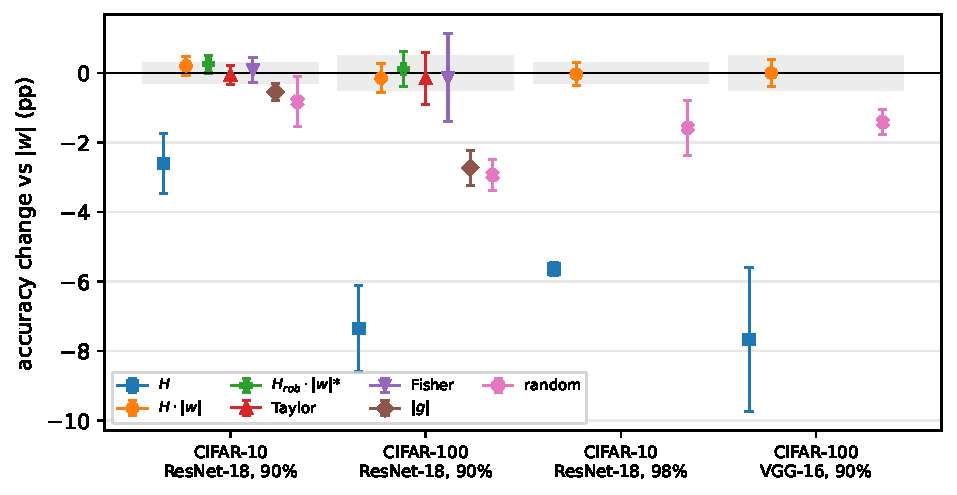
\includegraphics[width=0.9\textwidth]{Figures/penalty_by_regime.pdf}
\caption{Accuracy change of each criterion relative to $|w|$ (95\% Welch CI) in each regime. The grey band is the equivalence margin ($\pm0.3$ points on CIFAR-10, $\pm0.5$ on CIFAR-100). Open marker: exploratory criterion.}
\label{fig:penalty}
\end{figure*}

\paragraph{Difficulty (H3).} Fig.~\ref{fig:penalty} summarises Table~\ref{tab:regimes}. Every criterion that is far from $|w|$ loses more in the harder regimes than on CIFAR-10 at 90\%: entropy alone from $2.6$ to between $5.6$ and $7.7$ points, random from $0.8$ to between $1.4$ and $2.9$, gradient magnitude from $0.5$ to $2.7$. The number of criteria with a significant difference does not rise uniformly (2 of 6 on CIFAR-10 at 90\%, 3 of 6 on CIFAR-100, 1 of 3 at 98\%, 2 of 3 with VGG-16), partly because the secondary regimes test fewer criteria. H3 is supported for the size of the penalties and only partly for their number.

\paragraph{FLOPs.} Criteria that remove the same number of weights remove different amounts of computation, because they allocate the budget differently across layers. On CIFAR-10 at 90\%, $|w|$ removes 74.5\% of the non-zero FLOPs, $H\cdot|w|$ 73.4\%, Taylor and Fisher about 71\%, random 81.5\% and $H$ alone 86.0\%. The two worst criteria remove the most FLOPs, because they prune the early, high-resolution layers more (Fig.~\ref{fig:density}); none of these differences is realised as a speed-up with dense kernels.

\begin{figure*}[t]
\centering
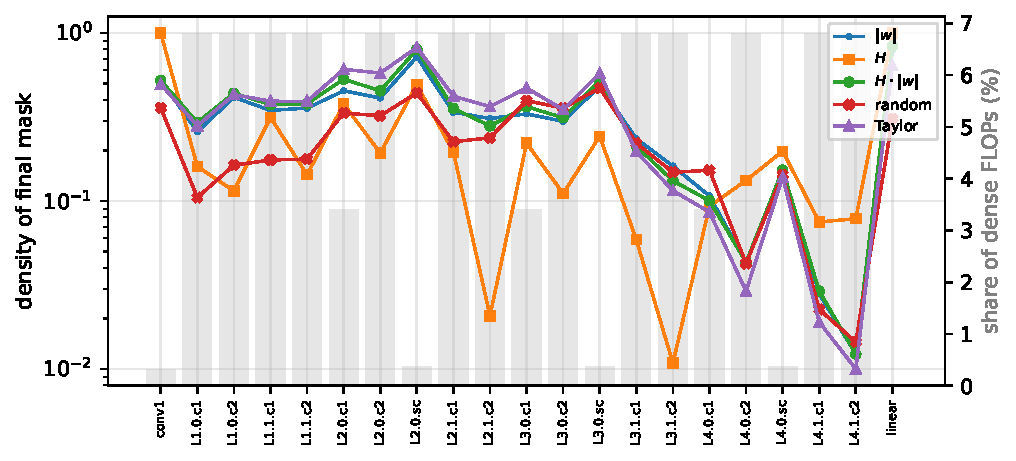
\includegraphics[width=0.9\textwidth]{Figures/layer_density_cifar10_resnet18_s90.pdf}
\caption{Density of the final mask per layer (log scale, mean over seeds) for several criteria, ResNet-18 on CIFAR-10 at 90\% sparsity. Grey bars: each layer's share of the dense FLOPs. All criteria keep the same total number of weights.}
\label{fig:density}
\end{figure*}

\subsection{Allocation or ranking? (H5)}
\label{sec:allocation}

Table~\ref{tab:allocation} repeats the ablation with a layer-uniform allocation, in which no criterion can move budget between layers.

\begin{table*}[t]
\centering
\caption{C0 criteria with global and layer-uniform allocation (CIFAR-10, ResNet-18, 90\%). With uniform allocation every layer keeps the same density, so differences can only come from which weights are dropped inside a layer.}
\label{tab:allocation}
\resizebox{\textwidth}{!}{%
\begin{tabular}{llcccccc}
\toprule
Allocation & Drop criterion & Acc (\%) & $\Delta$ vs $|w|$ [95\% CI] (pp) & $p_{\mathrm{Holm}}$ & Equiv. & FLOPs red.\ sparse (\%) & Seeds \\
\midrule
global & $|w|$ & 95.03 $\pm$ 0.07 & -- & -- & -- & 75.2 $\pm$ 1.5 & 3 \\
global & $H(A)$ & 92.44 $\pm$ 0.40 & -2.59 [-3.55, -1.63] & 0.020 & no & 86.0 $\pm$ 0.7 & 3 \\
global & $H(A)\cdot|w|$ (DEGST) & 95.30 $\pm$ 0.21 & +0.27 [-0.20, +0.74] & 0.288 & no & 73.6 $\pm$ 0.7 & 3 \\
uniform & $|w|$ & 94.43 $\pm$ 0.08 & -- & -- & -- & 90.0 $\pm$ 0.0 & 3 \\
uniform & $H(A)$ & 91.63 $\pm$ 0.37 & -2.80 [-3.67, -1.93] & 0.017 & no & 90.2 $\pm$ 0.0 & 3 \\
uniform & $H(A)\cdot|w|$ (DEGST) & 94.72 $\pm$ 0.23 & +0.29 [-0.21, +0.79] & 0.288 & no & 90.0 $\pm$ 0.0 & 3 \\
\bottomrule
\end{tabular}}
\par\smallskip\footnotesize Mean $\pm$ std over 3 seeds; $^{*}$ marks single-seed cells (no std); -- = not yet run. Accuracy is final-epoch test accuracy. $\Delta$: difference of means to the $|w|$ row of the same block, with its 95\% Welch CI; $p_{\mathrm{Holm}}$: two-sided Welch test, Holm-adjusted over all confirmatory comparisons of the table; Equiv.: TOST at $\pm$0.3 pp (CIFAR-10) / $\pm$0.5 pp (CIFAR-100, Tiny ImageNet), $\alpha$ = 0.05. Exploratory rows are not in the Holm family (unadjusted $p$). Measured sparsity of $H(A)$ (uniform): 90.17--90.33\%, because weights regrown where the gradient is exactly zero (inputs from dead channels) stay zero.
\end{table*}


Entropy alone remains $2.80$ points below $|w|$ ($[-3.67,-1.93]$), compared with $2.59$ points under global allocation, so H5 is not supported: its loss comes from which weights it drops inside each layer, not from the allocation. This also rules out a second explanation suggested by Fig.~\ref{fig:density}: under global allocation, entropy alone keeps the first convolution and the classifier dense but drives two middle layers down to 1--2\% density, close to the per-layer floor. With uniform allocation no layer can be starved in this way, and the loss remains. $H\cdot|w|$ is again not significantly different from $|w|$ ($+0.29$, $[-0.21,+0.79]$). Uniform allocation costs $|w|$ itself $0.6$ points while removing more FLOPs (90\% instead of 75\%). With uniform allocation, entropy alone ends at 90.2--90.3\% measured sparsity instead of 90.0\%: every layer must regrow its own quota, and weights regrown where the gradient is exactly zero (inputs from dead channels) stay zero. This makes its effective budget 2--3\% smaller, far too little to account for a gap of almost three points.

\subsection{How far is each criterion from magnitude? (H4)}
\label{sec:divergence}

Fig.~\ref{fig:divergence} plots each criterion's accuracy change against its divergence from $|w|$.

\begin{figure}[t]
\centering
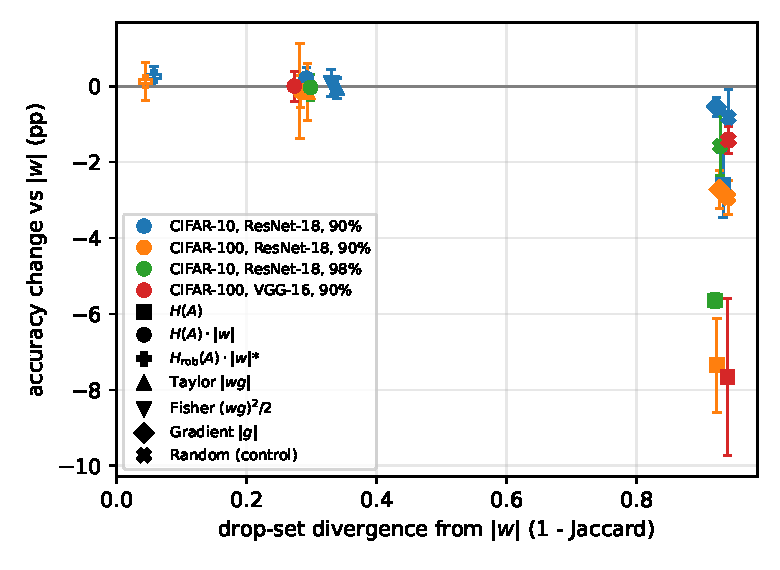
\includegraphics[width=\linewidth]{Figures/divergence_accuracy.pdf}
\caption{Accuracy change relative to $|w|$ (with 95\% CI) against the drop-set divergence $1-J$ from $|w|$, measured by replaying the loop's updates at epochs 50 and 100 (Sec.~\ref{sec:overlap}). Colours: regimes; markers: criteria; open markers: exploratory.}
\label{fig:divergence}
\end{figure}

The pre-specified test supports H4: Spearman $\rho=-0.70$ over the 18 confirmatory points ($p=0.001$). The figure shows, however, that the divergences fall into two clusters rather than along a continuum. $H\cdot|w|$, Taylor and Fisher drop sets differ from that of $|w|$ with divergences between 0.27 and 0.34, and their accuracy changes lie between $-0.15$ and $+0.21$ points, none of them significant. $H$ alone, $|g|$ and random share almost nothing with $|w|$ (divergences 0.92--0.94) and lose between $0.54$ and $7.67$ points. Within that far cluster the divergence is nearly constant while the loss varies fourteen-fold, so the divergence does not explain it. The correlation therefore mostly reflects the near/far split; the points also share regimes and the $|w|$ reference, so the $p$-value is optimistic (post hoc: within-regime $\rho$ is $-0.94$ and $-0.83$ in the two main regimes with six points each, and $-0.50$ in the secondary regimes with three). We read the result as a tolerance rather than a dose--response: the loop absorbs a change of about a third of the dropped weights at no measurable cost, while criteria that ignore magnitude altogether lose accuracy by an amount that depends on the criterion.

\subsection{What the entropy score measures}
\label{sec:what-h}

\paragraph{Entropy alone is worse than random (post hoc).} At the same divergence from $|w|$, entropy alone loses far more than a random drop. Table~\ref{tab:hrandom} compares the two directly.

\begin{table*}[t]
\centering
\caption{Post hoc comparison: drop by entropy alone against random drop, same loop and regrowth. Both drop sets overlap with that of $|w|$ by less than 10\% (Fig.~\ref{fig:divergence}).}
\label{tab:hrandom}
\resizebox{\textwidth}{!}{%
\begin{tabular}{lcccc}
\toprule
Regime & $H(A)$ (\%) & Random (\%) & $\Delta$ $H(A) -$ random [95\% CI] (pp) & $p_{\mathrm{Holm}}$ \\
\midrule
CIFAR-10, ResNet-18, 90\% & 92.44 $\pm$ 0.40 & 94.23 $\pm$ 0.35 & -1.79 [-2.64, -0.93] & 0.009 \\
CIFAR-100, ResNet-18, 90\% & 69.24 $\pm$ 0.57 & 73.65 $\pm$ 0.22 & -4.41 [-5.65, -3.18] & 0.007 \\
CIFAR-10, ResNet-18, 98\% & 88.13 $\pm$ 0.08 & 92.21 $\pm$ 0.35 & -4.07 [-4.89, -3.25] & 0.006 \\
CIFAR-100, VGG-16, 90\% & 66.28 $\pm$ 0.87 & 72.53 $\pm$ 0.18 & -6.25 [-8.29, -4.21] & 0.009 \\
\bottomrule
\end{tabular}}
\par\smallskip\footnotesize Welch tests, Holm-adjusted over the regimes shown. This comparison was not planned before the results; it is reported as a post hoc analysis.
\end{table*}


Entropy alone is worse than random in every regime, by $1.8$ to $6.3$ points ($p_{\mathrm{Holm}}<0.01$). It is not merely uninformative; it is misleading.

\paragraph{Entropy measures sparsity.} In the replay, the entropy of a channel is strongly anti-correlated with its share of exact zeros: Spearman $\rho$ between $-0.61$ and $-0.93$ over all channels after the first layer, at every checkpoint (Fig.~\ref{fig:hsparsity}). After a ReLU, most of a sparse channel's values fall into the first histogram bin, so its entropy is low. Ranking by low entropy therefore removes the weights that read the sparsest channels. That this is worse than random suggests that these channels, silent on most inputs, carry selective, discriminative responses, which a histogram entropy counts as uninformative. The correlation is measured; the interpretation is our explanation of it.

\begin{figure*}[t]
\centering
\IfFileExists{Figures/entropy_vs_sparsity.pdf}{%
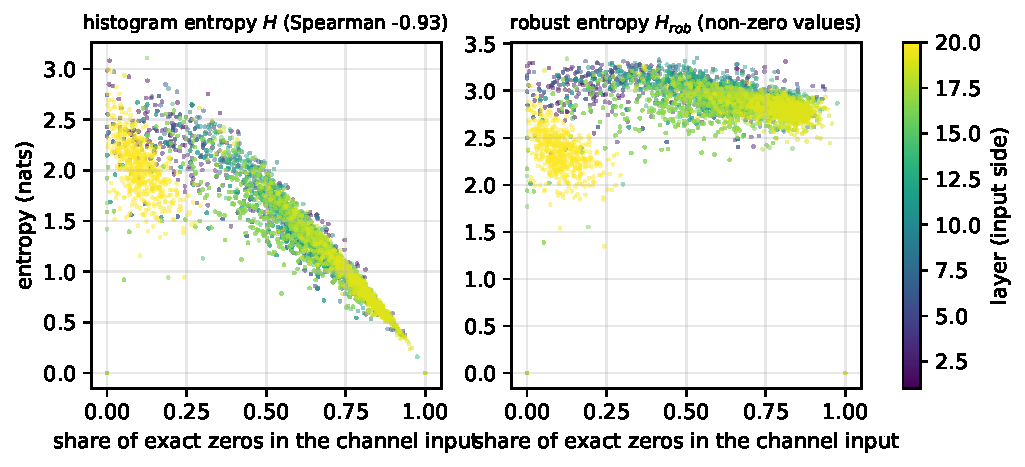
\includegraphics[width=0.9\textwidth]{Figures/entropy_vs_sparsity.pdf}}{%
\fbox{\parbox{0.8\textwidth}{\centering\vspace{2em}Figure pending: run \texttt{analysis/score\_overlap.py} on the epoch-50 checkpoint with \texttt{--out-dir results/analysis\_channels}, then \texttt{aggregate.py}.\vspace{2em}}}}
\caption{Per-channel entropy of the input of every layer after the first against the share of exact zeros in that input, ResNet-18 on CIFAR-100 at 90\% sparsity, epoch 50. Left: the histogram entropy used by the criteria. Right: the robust estimate over non-zero values. Colour: layer depth.}
\label{fig:hsparsity}
\end{figure*}

\paragraph{A robust estimate (exploratory).} $H_{\mathrm{rob}}\cdot|w|$ removes the zeros and outliers from the estimate. Its drop sets are almost those of $|w|$ (divergence 0.04--0.07): once zeros are excluded, the entropy varies little across the channels of a layer and hardly changes the ranking. Its difference to $|w|$ is $+0.26$ points on CIFAR-10 ($[+0.01,+0.52]$, unadjusted $p=0.047$) and $+0.12$ on CIFAR-100 ($[-0.39,+0.63]$). Given how little it changes the drop sets and that the result does not repeat on CIFAR-100, we do not interpret the CIFAR-10 difference.

\section{Discussion}
\label{sec:discussion}

\paragraph{How much does the drop criterion matter?} Less than its role in the loop suggests, as long as it stays close to magnitude. Replacing about a third of magnitude's drop decisions, with an entropy weighting or with a loss-based Taylor or Fisher score, changed accuracy by at most a few tenths of a point in every regime, never significantly, and for entropy-weighted magnitude, tested with five seeds, the change was within the equivalence margin in three of the four regimes. The loop is tolerant: weights dropped by mistake can be regrown by gradient at the next update, and at moderate sparsity many sub-networks of the same size train equally well. What the loop does not tolerate is a criterion that ignores magnitude. Such criteria share almost none of magnitude's choices and lose accuracy, more so as the task becomes harder: the gap between the best and the worst criterion is about three points on CIFAR-10 at 90\% sparsity but seven to eight on CIFAR-100.

\paragraph{Relation to earlier comparisons.} Our results agree with Nowak et al.\ \cite{nowak2023fantastic} that magnitude is hard to beat at low density, and that criteria which make similar decisions perform alike. One result differs: in their comparison, the SNIP-like score $|w|\cdot|g|$ fell behind magnitude at low density, whereas our Taylor score, the same product, is indistinguishable from $|w|$ at 10\% density. A likely reason, which we have not tested, is that we average $|w\,g|$ over the $\Delta T=400$ steps between updates, which removes much of the mini-batch noise of the gradient; they also report that frequent updates hurt the criteria that use gradients. Our gradient-only score $|g|$, which has no magnitude term, is clearly worse, consistent with the view that magnitude is the component that carries the drop decision.

\paragraph{Why the easy regime is a poor test bed.} On CIFAR-10 at 90\% sparsity, $|w|$ is within 0.3 points of the dense model and a random drop loses less than one point. Differences between reasonable criteria are then of the order of the seed-to-seed variation, which is where our one inconclusive result lies. Claims about drop criteria made only in this regime, including the one we set out to test, should be read with this ceiling in mind.

\paragraph{Why entropy fails as a drop score.} The failure of entropy alone is not a lack of signal but a misleading one: it is worse than a random drop in every regime. The replay offers an explanation. After a ReLU, the histogram entropy of a channel is dominated by its share of zeros, so low entropy marks the channels that are silent on most inputs. Such channels are not necessarily redundant; a channel that fires for few inputs can be the one that separates them. Entropy computed without the zeros varies little across channels and no longer changes the ranking. The original intuition, that a weight reading a near-constant input acts like a bias, holds for truly constant (dead) channels. In the replay they make up, on average per layer, 1--7\% of the input channels at 90\% sparsity and about a quarter at 98\%, but they do not need entropy to be found: a weight whose input is always zero receives no gradient and shrinks under weight decay, so magnitude drops it as well.

\paragraph{What this means for designing drop criteria.} A new drop score should be evaluated against magnitude in more than one regime, with a random-drop control to set the scale, and with a statement of how much its drop set differs from that of magnitude. A score that changes little is unlikely to matter; a score that changes a lot must earn its difference in accuracy, and activation statistics that are confounded with sparsity are a poor basis for it.

\section{Limitations}
\label{sec:limitations}

\begin{itemize}
    \item \textbf{Scale.} All regimes use $32\times32$ images (CIFAR-10/100). A Tiny ImageNet regime was prepared but not run. Rankings on CIFAR need not carry over to ImageNet \cite{deng2009imagenet}, where DST is usually evaluated \cite{evci2020rigging}.
    \item \textbf{One loop.} Regrowth is always by gradient magnitude, with one schedule and (except in Sec.~\ref{sec:allocation}) global allocation. Other regrowth rules, such as random regrowth \cite{mocanu2018scalable}, or other schedules may interact differently with the drop criterion. We did not run the reference RigL configuration (random ERK mask, no warm-up) alongside our loop.
    \item \textbf{Statistics.} Most cells have three seeds, which gives wide intervals: several loss-based criteria and the CIFAR-10 random control can be neither separated from $|w|$ nor shown equivalent. The equivalence claim rests on five seeds. Dense references have one seed. The comparison of entropy with random and the robustness checks of H4 were added after the results were seen and are labelled post hoc.
    \item \textbf{Divergence.} Drop-set overlaps are measured on the trajectory of the $|w|$ run (one seed) at two checkpoints, with the weights frozen during the replay; a criterion's own trajectory could drift further. The explanation of the entropy result by post-ReLU sparsity rests on a correlation.
    \item \textbf{Run-to-run variation.} Training is not bitwise deterministic. A first run of the C0 ablation gave $-0.04$ points for $H\cdot|w|-|w|$, the re-run $+0.27$; both are below the pre-specified threshold, and all reported numbers come from the re-run.
    \item \textbf{Hardware.} Unstructured sparsity is executed with dense kernels; we report non-zero FLOPs but no speed-ups.
\end{itemize}

\section{Conclusion}
\label{sec:conclusion}

We set out to improve the drop criterion of dynamic sparse training with activation entropy and found that it did not help. Turning the question into a controlled study of eight criteria in four regimes, with hypotheses and equivalence margins fixed in advance, gave a clearer picture. Magnitude is a necessary part of the drop score: entropy alone loses 2.6 to 7.7 points, and it is worse than dropping at random, because the histogram entropy of a post-ReLU channel mostly measures its sparsity. Entropy-weighted magnitude is equivalent to magnitude in three of four regimes and inconclusive in the easiest one, and loss-based Taylor and Fisher scores are no different from magnitude either. The loop tolerates criteria that change about a third of magnitude's decisions, but not criteria that ignore magnitude, and the cost of ignoring it grows with task difficulty. Future work should test these findings at ImageNet scale, with other regrowth rules, and with criteria that combine magnitude with an explicit estimate of the loss increase.

\section*{Code and data availability}

The code of the training loop and of every criterion, the experiment plan, the design document with the hypotheses and its dated changelog, the result files of all runs and the scripts that produce every table and figure of this paper are available at \TODO{repository URL}.


% To print the credit authorship contribution details
\printcredits

%% Loading bibliography style file
%\bibliographystyle{model1-num-names}
\bibliographystyle{cas-model2-names}

% Loading bibliography database
\bibliography{cas-refs}

% Biography
%\bio{}
% Here goes the biography details.
%\endbio

%\bio{pic1}
% Here goes the biography details.
%\endbio

\end{document}

